\section{Procedimentos}
	Esta seção tem como objetivo relatar os procedimentos gerais da programação, por exemplo como ligar o robô, quais as funcionalidades que temos e como podemos modifica-las entre outros procedimentos. Lembrando sempre que tudo que relatarmos aqui não significam que sejam os modos mais eficientes ou da melhor forma, sempre questionem os métodos e pensem melhores maneiras para resolver os problemas, e quando encontrarem novas formas melhores, pois vão encontrar, alterem esse documentos.
	
	\subsection{Ligar os motores}
		Primeiramente devemos verificar se os motores estão com energia, para isso basta apenas conectar a bateria e colocar o botão de emergência na posição ON. Caso o motor esteja alimentado de forma correta, os LED's deles deverão acender e em seguida desligar. Caso isso não ocorra solicitar ajuda para a equipe de Elétrica.
		
		Com os motores alimentados (certifique-se de que o código está compilado) podemos então executar o nó dos motores de duas formas, sendo a primeira executando o comando \textit{motors} no terminal:
		
		\begin{figure}[H]
			\centering
			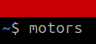
\includegraphics[scale=1]{sections/programacao/procedimentos/imagens/comando_motors.png}
		\end{figure}
		
	
		Ou indo até o diretório do RoboFEI e executando o comando \textit{source install/setup.bash} e na sequência o launch:
		
		\begin{figure}[H]
			\centering
			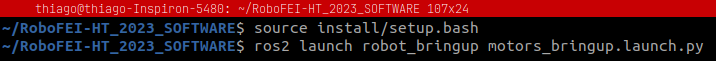
\includegraphics[scale=0.6]{sections/programacao/procedimentos/imagens/launch_motors.png}
		\end{figure}				
		
		
	\subsection{USB Rules}
		Como utilizamos mais de uma porta USB, uma para os motores e outra para a IMU foi necessário encontrarmos uma maneira de separar os USB's. Outro problema também que encontramos é que quando ligamos o USB o sistema do Linux não nos concede automaticamente permissão o suficiente para fazermos certas coisas, como por exemplo quando vamos executar o código dos motores, caso não seja dado permissão antes o código não consegue comunicar com os motores.
		
		Para tal problema podemos utilizar "Regras" para as USB, dessa forma podendo atribuir novos nomes e definir novas permissões, esse arquivo está contido no diretório do RoboFEI dentro de robot\_commands, e sua extensão é \textit{.rules}.
		
		\begin{figure}[H]
			\centering
			\caption{Exemplo de arquivo .rules}
			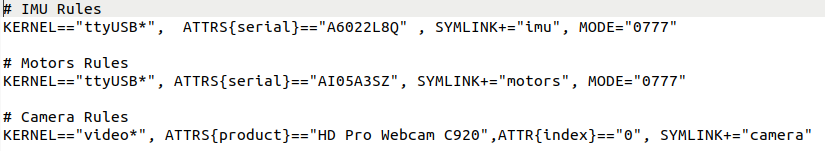
\includegraphics[scale=0.6]{sections/programacao/procedimentos/imagens/rules_file.png}
		\end{figure}
	
		Explicando um pouco mais do arquivo, inicialmente podemos ver que ambas as definições iniciam com o \textit{KERNEL} (é o responsável por controlar os periféricos do computador) \todo{citar https://www.significados.com.br/kernel/}, e nele vamos definir qual interface queremos modificar as regras. Para indicar o USB utilizamos o ttyUSB (em alguns sistemas se utilizam ttyACM), o simbolo de asterisco nos diz que iremos inicialmente selecionar todos os componentes que estão conectado ao USB, e idem para o video, mas que posteriormente serão filtrados de alguma maneira.
		
		Primeiramente analisando as linhas da IMU e dos motores, podemos ver na sequencia da especificação do \textit{KERNEL}, uma outra filtragem é utilizando o valor serial do USB, no nosso caso cada conversor que utilizamos possui um numero serial (podemos utilziar outros métodos para filtrar qual USB queremos encontrar), em seguida utilizamos o \textit{SYMLINK} para lincar a porta USB com um novo nome, e utilizamos \textit{MODE} para definir quais as permissões que precisamos para o USB.
		
		Utilizamos a mesma linha de raciocínio para a câmera, porem utilizamos o nome do produto e o \textit{index} para definirmos onde qual a interface que queremos modificar.
		
		Os procedimentos que devemos seguir caso precisemos alterar as rules é inicialmente saber qual interface o dispositivo está conectado, eles ficam todos situados no diretório \textit{/dev} (podendo ser por exemplo ttyUSB, video, entre outros). sabendo qual a interface podemos usar o comando:
		
		\begin{figure}[H]
			\centering
			\caption{Exemplo utilizando a interface \textit{video}}
			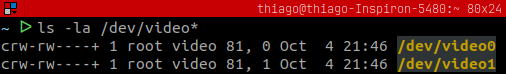
\includegraphics[scale=0.6]{sections/programacao/procedimentos/imagens/interface_list.png}
		\end{figure}
		
		Na sequencia podemos ver as informações dessa interface como mostra a imagem abaixo.
		
		\begin{figure}[H]
			\centering
			\caption{Informações da interface \textit{video}}
			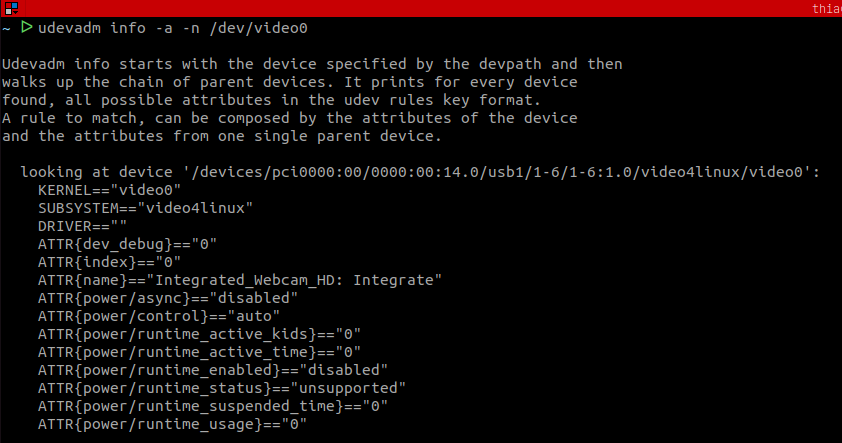
\includegraphics[scale=0.5]{sections/programacao/procedimentos/imagens/interface_info.png}
		\end{figure}
	
		Como podemos ver, cada interface tem sua combinação de informações e utilizando elas podemos separar a interface que queremos utilizar.
		
		Após criar o arquivo \textit{.rules} com as suas necessidades, basta copiar o arquivo para o diretório \textit{/etc/udev/rules.d}
		e em seguida realizar a sequencia de comandos:
		
		\begin{figure}[H]
			\centering
			\caption{Reiniciar as regras de interface \textit{video}}
			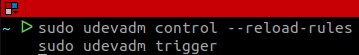
\includegraphics[scale=0.5]{sections/programacao/procedimentos/imagens/reload_rules.png}
		\end{figure}
		
		Caso tenha ocorrido tudo certo, suas regras já estarão funcionando, e você pode verificar elas usando o comando \textit{ls -la /dev/\{novo nome interface\}}. 
		
		Caso fique alguma dúvida pode-se utilizar o link https://dev.to/enbis/how-udev-rules-can-help-us-to-recognize-a-usb-to-serial-device-over-dev-tty-interface-pbk, onde possui uma melhor explicação do assunto e uma outra abordagem para realizar esse processo.		

\subsection{Comandos personalizados no terminal}		

\subsection{Servidor UDP}
FAZER

\subsection{Conectar Wi-Fi}
FAZER
